\chapter{RESULTS}
The updated design brings together footstep energy harvesting, phone-based location tracking and emergency lighting. The reported tests give initial results for current draw, SOS operation, heat and water exposure. The following sections discuss what these results mean in use, while keeping calculated estimates and intended functions separate from measured performance.

\section{Energy Use and Operating Time}
The main 3.7~V, 4000~mAh battery has a nominal capacity of 14.8~Wh. It supplies the on-shoe electronics and stores energy collected from footsteps~\cite{ahmed2024smart}. The current readings show that the choice of lighting mode has a clear effect on demand, as summarised in Table~\ref{tab:current_draw_steady_lighting}.

\begin{table}[H]
    \centering
    \caption{Reported current draw in the steady lighting modes}\label{tab:current_draw_steady_lighting}
    \begin{tabularx}{\textwidth}{
        >{\hsize=0.50\hsize\raggedright\arraybackslash}X
        >{\hsize=1.80\hsize\raggedright\arraybackslash}X
        >{\hsize=0.7\hsize\raggedright\arraybackslash}X
    }
    \toprule
    \textbf{Mode} & \textbf{Lighting output} & \textbf{Current} \\
    \midrule
    Mode 1 & Front white LEDs only & About 60 mA \\
    \addlinespace
    Mode 2 & Front LEDs and cyan/white strip at 30\% brightness & About 140 mA \\
    \bottomrule
    \end{tabularx}
\end{table}

Adding the strip increases the reported current by about 80~mA, making Mode 2 draw roughly 2.3 times as much as Mode 1. The extra light around the shoe therefore comes with a noticeable increase in battery demand. Current readings for standby, flashing and SOS are not given, so their operating times cannot be compared in the same way.

If the Mode 2 reading represents the total battery current, a simple capacity estimate gives:
\begin{equation}
    t = \frac{4000 \text{ mAh}}{140 \text{ mA}} \approx 28.6 \text{ h}
    \label{eq:battery_time}
\end{equation}

To highlight this power-runtime trade-off, Figure~\ref{fig:power-barchart} compares the reported current draw and resulting ideal battery duration for both steady lighting modes.

\begin{figure}[htbp]
    \centering
    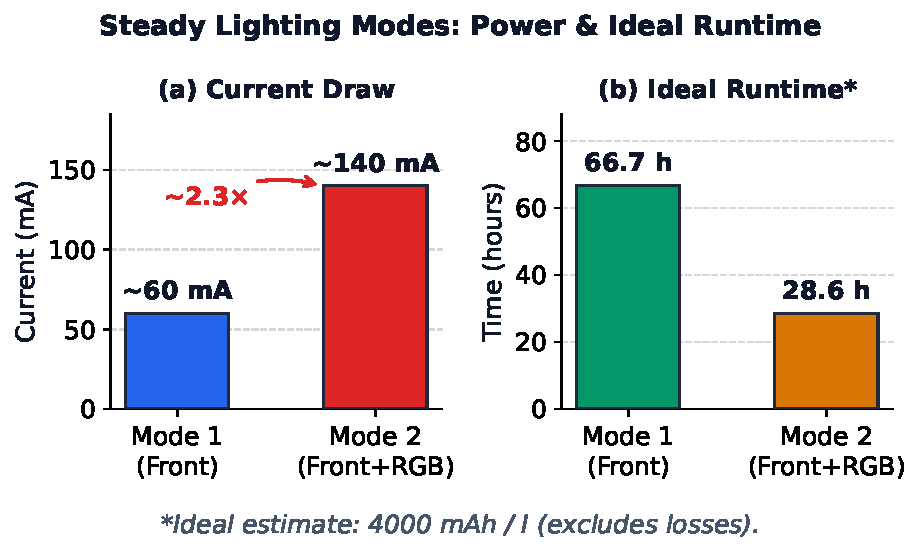
\includegraphics[scale=0.9]{figures/power_barchart.pdf}
    \caption{Comparison of reported steady-state current draw and ideal battery runtime between 2 modes}\label{fig:power-barchart}
\end{figure}

This is consistent with the scale of the reported range. It is an ideal estimate, however, and assumes the full rated capacity is available at a constant current. Circuit losses, the usable discharge range and the measurement point still need to be considered. The 24--30-hour figure should therefore not be treated as a verified duration for every mode.

Footstep harvesting could extend operating time, but the source does not state how much energy actually reaches the battery. The PVDF output voltage alone cannot answer this. Over a given period, the relevant balance is:
\begin{equation}
    \Delta E = H - L
    \label{eq:energy_balance}
\end{equation}

Here, $\Delta E$ is the change in stored battery energy, $H$ is the energy added after harvesting and charging losses, and $L$ is the energy taken from the battery by the electronics, including supply losses. If $H$ is smaller than $L$, the battery still discharges while the user walks. Without these measurements, continuous operation from footsteps alone has not been demonstrated.

\section{AI-Assisted Positioning and SOS}
The updated app changes how location tracking is managed. Instead of using the same GPS activity all the time, it uses the phone's motion sensors and BLE information to adjust tracking to the user's situation. Table~\ref{tab:GPS_behaviour_app} shows the intended behaviour. These functions run on the smartphone; they do not require a separate GPS receiver inside the shoe.

\begin{table}[H]
    \centering
    \caption{Intended GPS behaviour in the updated app}\label{tab:GPS_behaviour_app}
    \begin{tabularx}{\textwidth}{
        >{\hsize=0.50\hsize\raggedright\arraybackslash}X
        >{\hsize=1.30\hsize\raggedright\arraybackslash}X
        >{\hsize=1.20\hsize\raggedright\arraybackslash}X
    }
    \toprule
    \textbf{Situation} & \textbf{App response} & \textbf{Purpose} \\
    \midrule
    User is still & Reduce GPS update frequency. & Limit unnecessary phone battery use~\cite{android_location_battery}. \\
    \addlinespace
    Walking or running & Increase updates and filter implausible location jumps. & Keep the displayed route more useful during movement. \\
    \addlinespace
    SOS is activated & Switch to high-accuracy GPS and send live coordinates to saved contacts. & Prioritise location information for the emergency alert. \\
    \bottomrule
    \end{tabularx}
\end{table}

Filtering is intended to reduce sudden GPS jumps in crowded urban areas or partly indoors~\cite{weng2023gnss}. The source reports accurate live tracking and reduced battery use during the SOS workflow test, but gives no location-error measurements or comparison with ordinary GPS tracking. These are qualitative findings: the amount of improvement, and the contribution of the AI feature itself, remain unmeasured. Any saving from changing GPS activity concerns the phone battery, rather than directly proving a longer shoe runtime.

The reported SOS test also found that holding the button for 3 seconds prevented accidental alarms during running or jumping, and that BLE reliably reached the phone at normal walking distances. The app was reported to send the emergency message quickly. These observations support the basic workflow under the described conditions, although no trial count, exact distance or delivery time is provided.

A single SOS request produces two useful outputs: a visible warning nearby and a location message for a saved contact. The lights can attract attention, while the phone provides the location and Internet connection needed for the remote alert. Seeing the red SOS pattern does not itself confirm message delivery. The emergency request remains button-activated; motion sensing in the app manages GPS updates and is not described as automatic fall detection.

\section{Lighting and Physical Test Results}
The lighting modes offer a choice between lighting the path ahead and making the shoe more visible from the sides. Table~\ref{tab:lighting_emergency} summarises the programmed responses, including the emergency override.

\begin{table}[H]
    \centering
    \caption{Lighting modes and emergency response}\label{tab:lighting_emergency}
    \begin{tabularx}{\textwidth}{
        >{\hsize=0.7\hsize\raggedright\arraybackslash}X
        >{\hsize=1.3\hsize\raggedright\arraybackslash}X
    }
    \toprule
    \textbf{Mode} & \textbf{Programmed lighting response} \\
    \midrule
    Mode 0: Standby & All lights are off. \\
    \addlinespace
    Mode 1: Front light & Front white LEDs light the path ahead. \\
    \addlinespace
    Mode 2: Front and strip & Front LEDs remain on; the strip glows cyan/white at 30\% brightness. \\
    \addlinespace
    Mode 3: Flashing & Lights flash at 2~Hz (twice per second). \\
    \addlinespace
    Emergency SOS & Normal modes are overridden. Front LEDs flash rapidly and the strip displays red Morse-code SOS at full brightness. \\
    \bottomrule
    \end{tabularx}
\end{table}

Short presses cycle through the normal modes, while a 50~ms debounce filter helps prevent one press from being read as several inputs. Once SOS is activated, its light pattern takes priority over the current mode.

The physical tests focused on heat build-up and water entering around the exposed parts. Table~\ref{tab:heat_water_exposure} brings together the reported conditions and observations.

\begin{table}[H]
    \centering
    \caption{Reported heat and water-exposure test results}\label{tab:heat_water_exposure}
    \begin{tabularx}{\textwidth}{
        >{\hsize=0.50\hsize\raggedright\arraybackslash}X
        >{\hsize=1.30\hsize\raggedright\arraybackslash}X
        >{\hsize=1.20\hsize\raggedright\arraybackslash}X
    }
    \toprule
    \textbf{Test} & \textbf{Condition} & \textbf{Reported observation} \\
    \midrule
    Heat & Two hours of continuous lighting inside a closed box. & The resistor, transistor and LED strip remained below 40 °C. \\
    \addlinespace
    Water exposure & Simulated rain and shallow puddles. & No leaks were reported around the front lens, side strip or collar button. \\
    \bottomrule
    \end{tabularx}
\end{table}

The heat test provides an initial check of the enclosed lighting components, while the water test supports the sealing at the inspected points under the stated conditions. Battery temperature, longer operating periods and repeated bending were not separately assessed. These observations therefore do not establish long-term durability or an IP67 rating for the complete shoe~\cite{iec60529}.

No visibility-distance measurements are available. Carbon fibre and titanium are also mentioned in the design overview, but no weight, strength or comfort results are supplied, so their practical benefits still need to be checked.

\section{Validation Priorities}
The next priority is to measure harvested energy and battery consumption over the same walking session, then run full discharge tests for each lighting mode. This would show whether footsteps meaningfully extend operating time. The GPS feature also needs comparison with a fixed-update setting, recording location error, phone battery use and the time from button activation to message delivery.

Before wider testing, the roles and interconnection of the nRF52832 SOS module and ESP32-C3 lighting controller should be clarified. Repeated bending, wet-use and wear tests would then check whether the wiring, seals and proposed protective materials remain practical in a shoe. These steps develop the functions already included in the updated design rather than adding further features.
